\documentclass[a4paper,11pt]{jsarticle}


% 数式
\usepackage{amsmath,amsfonts,amssymb}
\usepackage{bm}
% 画像
\usepackage[dvipdfmx]{graphicx}
\usepackage[dvipdfmx]{color}
\usepackage{siunitx}
\usepackage{wrapfig}
\usepackage{cases}
\usepackage{dcolumn}
\usepackage{subcaption}


% add hyperlinks
\usepackage[dvipdfmx]{hyperref}
\usepackage{pxjahyper}
\hypersetup{
  colorlinks=true,
  linkcolor=blue,
  citecolor=blue,
  breaklinks=true, 
}

% next page in align
\allowdisplaybreaks[1]

\begin{document}

\title{単振り子の長さと回転数の関係について}
\author{Hiro Hirabayashi}
\date{\today}
\maketitle

\begin{figure}[h]
  \begin{tabular}{cc}
    \begin{minipage}[t]{0.5\textwidth}
      \centering
      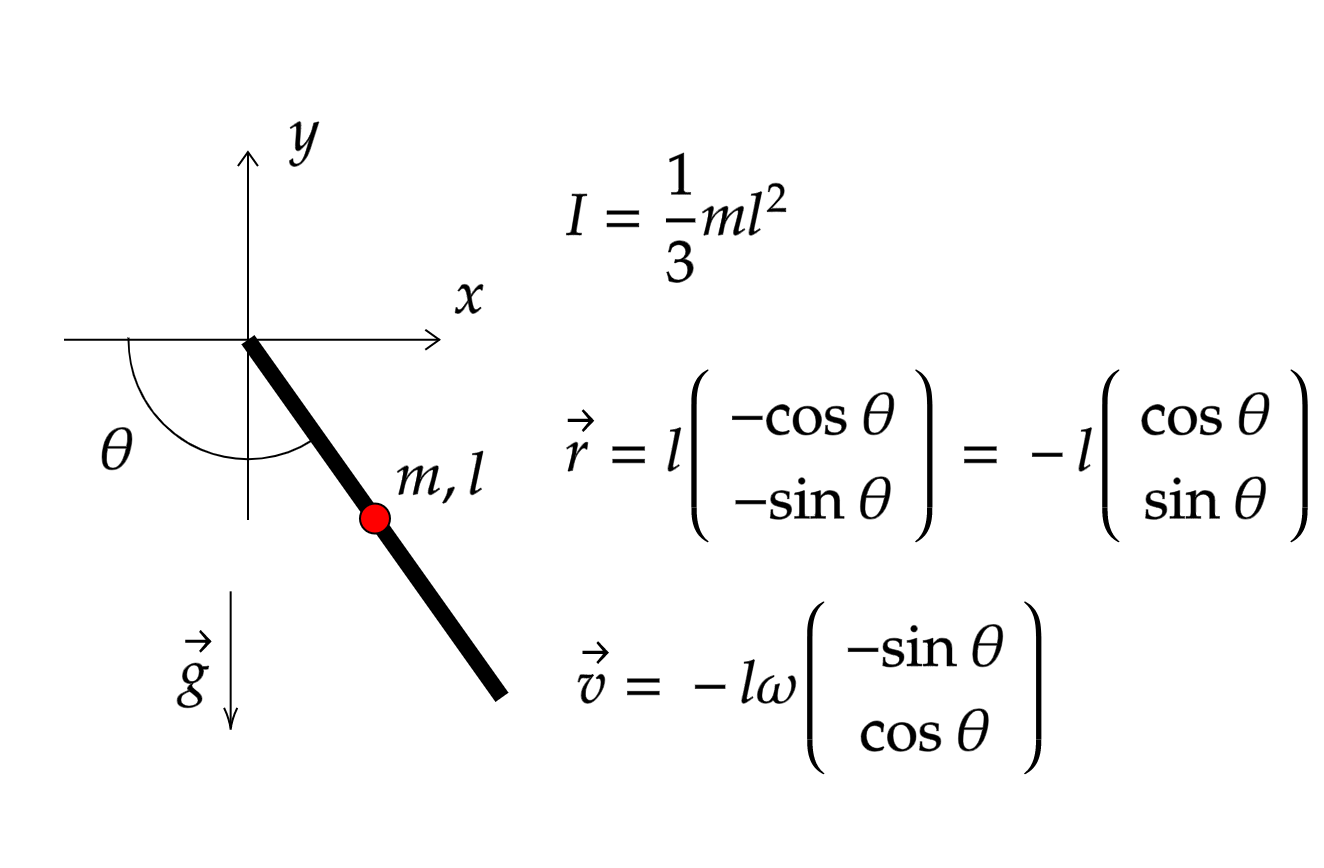
\includegraphics[width=1\textwidth]{config.png}
      \caption{設定}
      \label{config.png}
    \end{minipage} &
    \begin{minipage}[t]{0.5\textwidth}
      \centering
      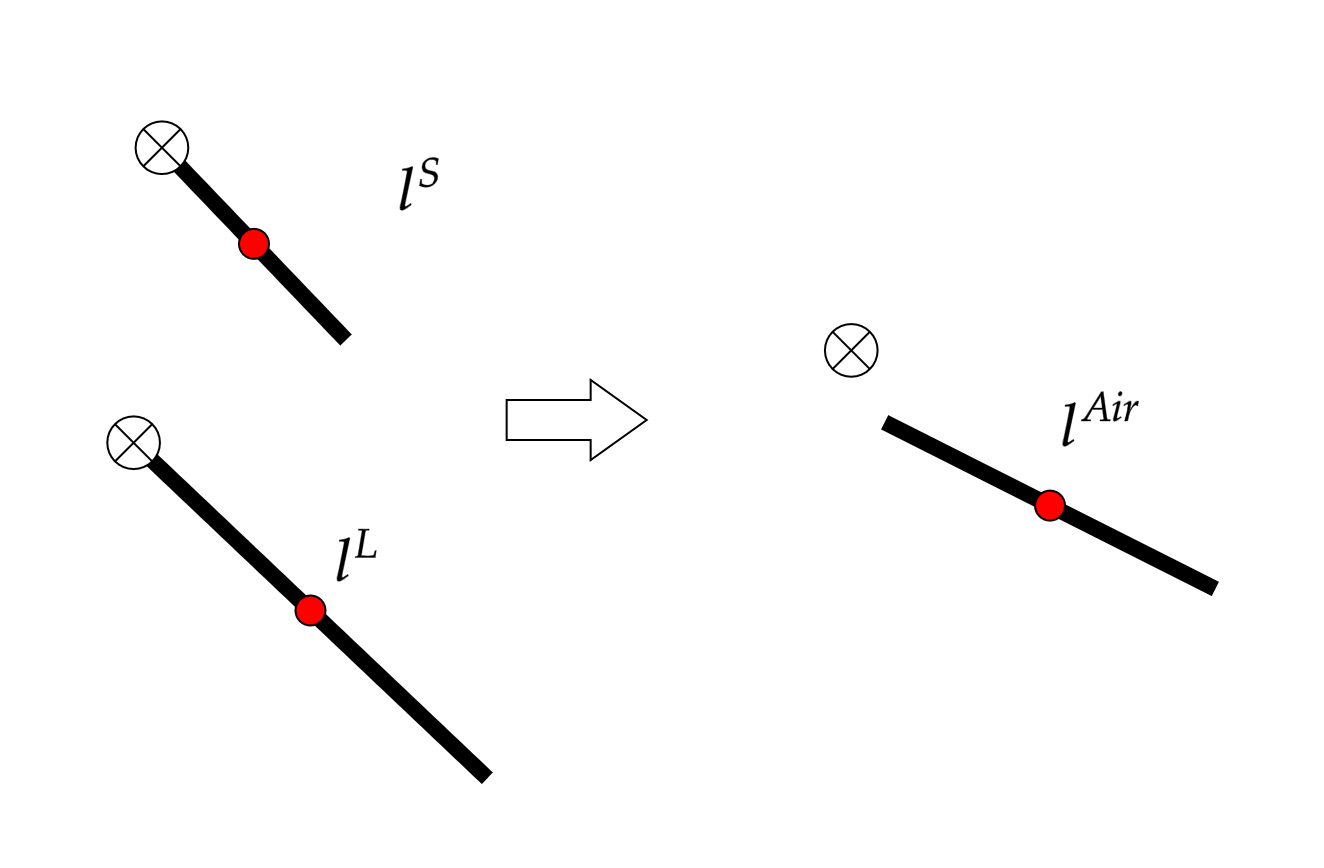
\includegraphics[width=1\textwidth]{length_after_takeoff.png}
      \caption{離軸後の慣性モーメント}
      \label{length_after_takeoff.png}
    \end{minipage}
  \end{tabular}
\end{figure}

図\ref{config.png}のような状況で、剛体振り子が回転軸から離れる状況を考える。
ただし、回転軸から離れた後は図\ref{length_after_takeoff.png}のように、
離軸前の振り子の長さ($l^L, l^S$)によらず、$l^{Air}$に変化する。
これは平行棒の後方宙返りにおいて、離手後に同じ姿勢をとる状況を再現するためである。
そしてこの文書は
"単振り子は長いほうが高い回転数を実現する"
ことを証明する文書である。

単振り子の良い点は、時間パラメータ$t$に対して解析的な解を求めなくても、
角度パラメータ$\theta$に対して簡単に解析的な解が求められることである。
2重振り子にはないこの特性は、
簡単に立てられるエネルギー保存則に含まれる変数が$\theta$とその微分である$\omega$
だけであることによる。

そして今回は、質量が一定に保たれ、密度が一様な剛体振り子を考えるが、
力学的エネルギーを長さ$l$によらず一定に保つために、
水平$\theta = 0$から振り出すことを考える。
するとエネルギーの保存則より
\begin{align}
  0 
  &= \frac{1}{2} m \Big\{ (l\omega\sin\theta)^2 + (-l\omega\cos\theta)^2  \Big\}
  + \frac{1}{2} \cdot \frac{1}{3} ml^2 \cdot \omega^2
  + mg (-l \sin\theta )
  \\
  &= \frac{1}{2}ml^2\omega^2 + \frac{1}{6}ml^2\omega^2 + mg (-l\sin\theta)
  \\
  &= \frac{2}{3}ml^2\omega^2 + mg (-l\sin\theta)
\end{align}
これにより
\begin{align}
  \omega^2 = \frac{3}{2ml^2}mgl\sin\theta = \frac{3g}{2l}\sin\theta
\end{align}
が求まる。
空中での回転速度を$\Omega$とすると
\begin{align}
  I\Omega 
  &= \frac{1}{3}ml^2\omega
  = \frac{1}{3}ml^2 \sqrt{ \frac{3g}{2l}\sin\theta }
  = \sqrt{ \frac{m^2 g}{6} l^3 \sin\theta }
\end{align}
\begin{align}
  \therefore \Omega
  &= \frac{1}{I} \sqrt{ \frac{m^2 g}{6} l^3 \sin\theta }
  \label{eq:Omega}
\end{align}

ところで、回転数$N_r$は滞空時間$T_{air}$、空中での回転速度$\Omega$を用いて
\begin{align}
  N_r = \Big( \theta + T_{air} \cdot \Omega \Big) / 2\pi
\end{align}
で表される。
"単振り子は長いほうが高い回転数を実現する"
ことを証明するには
例えば$\theta, \Omega$が同じ状況で、
$T_{air}$が長さに対して単調増加することを示せばよいが、
それは証明できない。
そもそも$\theta, \Omega$が同じ状況が用意できないが、
例えば$\theta=\frac{1}{2}\pi$での離軸を考えると良い。
振り子が短いほうが$T_{air}$は大きいが、
振り子が長いほうが$\Omega$は大きかったりする。
しかし、
離軸後の最高到達点の高さが一定である場合、
$\theta, T_{air}, \Omega$が
長さ$l$に対して単調増加することが示せる。

離軸後の最高到達点の高さが一定であるような条件は
鉛直方向のエネルギー保存を考えると簡単に表される。
離軸後の最高到達点の高さを$h$とする。
振り子は力学的エネルギーがすべて位置エネルギーに変換された場合の高さ$0$を超えることはないので、
$h\leq0$が成り立つ。
\begin{align}
  mgh 
  &= \frac{1}{2}m (-l \omega \cos \theta)^2 + mg (-l \sin \theta)
  \label{eq:energy_vertical}
  \\
  &= \frac{1}{2}ml^2 \omega^2 \cos^2 \theta + mg (-l \sin \theta)
  \\
  & \ \ \left( \because \omega^2 = \frac{3}{2ml^2}mgl\sin\theta = \frac{3g}{2l}\sin\theta \right) \notag
  \\
  &= \frac{1}{2}ml^2 \cos^2 \theta \cdot \frac{3g}{2l}\sin\theta + mg (-l \sin \theta)
  \\
  &= \frac{3mgl}{4}\sin\theta \cos^2\theta + mg (-l\sin\theta)
  \\
  &= mgl\cos\theta \left( \frac{3}{4}\cos^2\theta - 1\right)
  \\
  & \ \ \left( \because \cos^2\theta = 1 - \sin^2\theta \right) \notag
  \\
  &= mgl\sin\theta \left( \frac{3}{4} - \frac{3}{4}\sin^2\theta - 1 \right)
  \\
  &= mgl\sin\theta \left( - \frac{3}{4}\sin^2\theta - \frac{1}{4} \right)
  \\
  &= -\frac{1}{4}mgl\sin\theta (3\sin^2\theta + 1)
\end{align}
よって長さ$l$と離軸角度に関して以下の式が得られる。
\begin{align}
  & mgh = \frac{1}{4}mgl \sin\theta (3\sin^2\theta + 1)
  \\
  \Leftrightarrow
  & l = \frac{4(-h)}{\sin\theta (3\sin^2\theta + 1)} \ \ \ \ \Big( > 0, \ \ \because -h > 0, \sin\theta > 0 \Big)
  \label{eq:l_vs_sin}
\end{align}

平行棒の後方宙返りを模すために$\frac{1}{2}\pi \leq \theta \leq \pi$で離軸することを考える。
この区間で$\sin\theta$は単調減少するから
$\sin\theta (3\sin^2\theta)$ も単調減少する。
長い剛体振り子に対応する変数Xを$X^L$、
短い剛体振り子に対応する変数Xを$X^S$と表すと、
\begin{align}
  l^S < l^L
\end{align}
であるから、
式\ref{eq:l_vs_sin}によって
\begin{align}
  \frac{1}{\sin\theta^S (3\sin^2\theta^S + 1)} &< \frac{1}{\sin\theta^L (3\sin^2\theta^L + 1)}
  \\
  \Leftrightarrow
  \sin\theta^S (3\sin^2\theta^S + 1) &> \sin\theta^L (3\sin^2\theta^L + 1)
  \\
  \Leftrightarrow
  \sin\theta^S &> \sin\theta^L
  \\
  \Leftrightarrow
  \theta^S &< \theta^L
\end{align}
が分かる。
離軸後の最高到達点の高さが一定であるような条件において
長さ$l$に対して離軸時の角度$\theta$が単調増加であることが示された。

また、滞空時間$T_{air}$は
\begin{align}
  T_{air} = (\textrm{離軸から最高高度到達まで}) + (\textrm{最高高度到達以降})
\end{align}
で表され、
最高高度到達以降は"離軸後の最高到達点の高さが一定"によって一致するから、
$T_{air}$の差異は離軸から最高高度到達までにかかる時間によって生じる。
離軸時の鉛直方向速度$v_y$は
\begin{align}
  v_y = l\omega (-\cos\theta) \ \ \ \ \Big( > 0, \ \ \because \cos\theta < 0 \Big)
\end{align}
によって現れるが、
離軸後の最高到達点の高さが一定であるような条件において
長さ$l$に対して$T_{air}$が単調増加することを証明するのに
特に$\theta, \omega$で表す必要はない。
鉛直方向に関するエネルギー保存則の式\ref{eq:energy_vertical}を$v_y$で書き換えると
\begin{align}
  mgh = \frac{1}{2}m{v_y}^2 + mg (-l \sin\theta)
\end{align}
\begin{align}
  \Leftrightarrow
  \frac{1}{2}m{v_y}^2
  &= mgh + mgl\sin\theta
  = mgh + mg\sin\theta\cdot\frac{4(-h)}{\sin\theta(3\sin^2\theta + 1)}
  \\
  &= mg\left\{ h + \frac{4(-h)}{3\sin^2\theta + 1} \right\}
\end{align}
\begin{align}
  {v_y}^2 = 2g(-h)\left\{ \frac{1}{3\sin^2\theta + 1} - 1 \right\}
\end{align}
よって
\begin{align}
  l^S &< l^L
  \\
  \Leftrightarrow
  \sin\theta^S &> \sin\theta^L
  \\
  \Leftrightarrow
  3\sin^2\theta^S + 1 &> 3\sin^2\theta^L + 1
  \\
  \Leftrightarrow
  \frac{1}{3\sin^2\theta^S + 1} &< \frac{1}{3\sin^2\theta^L + 1}
  \\
  \Leftrightarrow
  {v_y^S}^2 &< {v_y^L}^2
  \\
  \Leftrightarrow
  v_y^S &< v_y^L
  \\
  \Leftrightarrow
  T_{air}^S &< T_{air}^L.
\end{align}
よって
離軸後の最高到達点の高さが一定であるような条件において
長さ$l$に対して滞空時間$T_{air}$が単調増加であることが示された。

離軸後の最高到達点の高さが一定であるような条件において
長さ$l$に対して離軸時の角度$\theta$と滞空時間$T_{air}$が単調増加であることから、
図\ref{same_max_height.png}が描ける。
長い振り子のほうが、位置エネルギーをうまく活用している様子が見て取れる。

\begin{figure}[h]
  \centering
  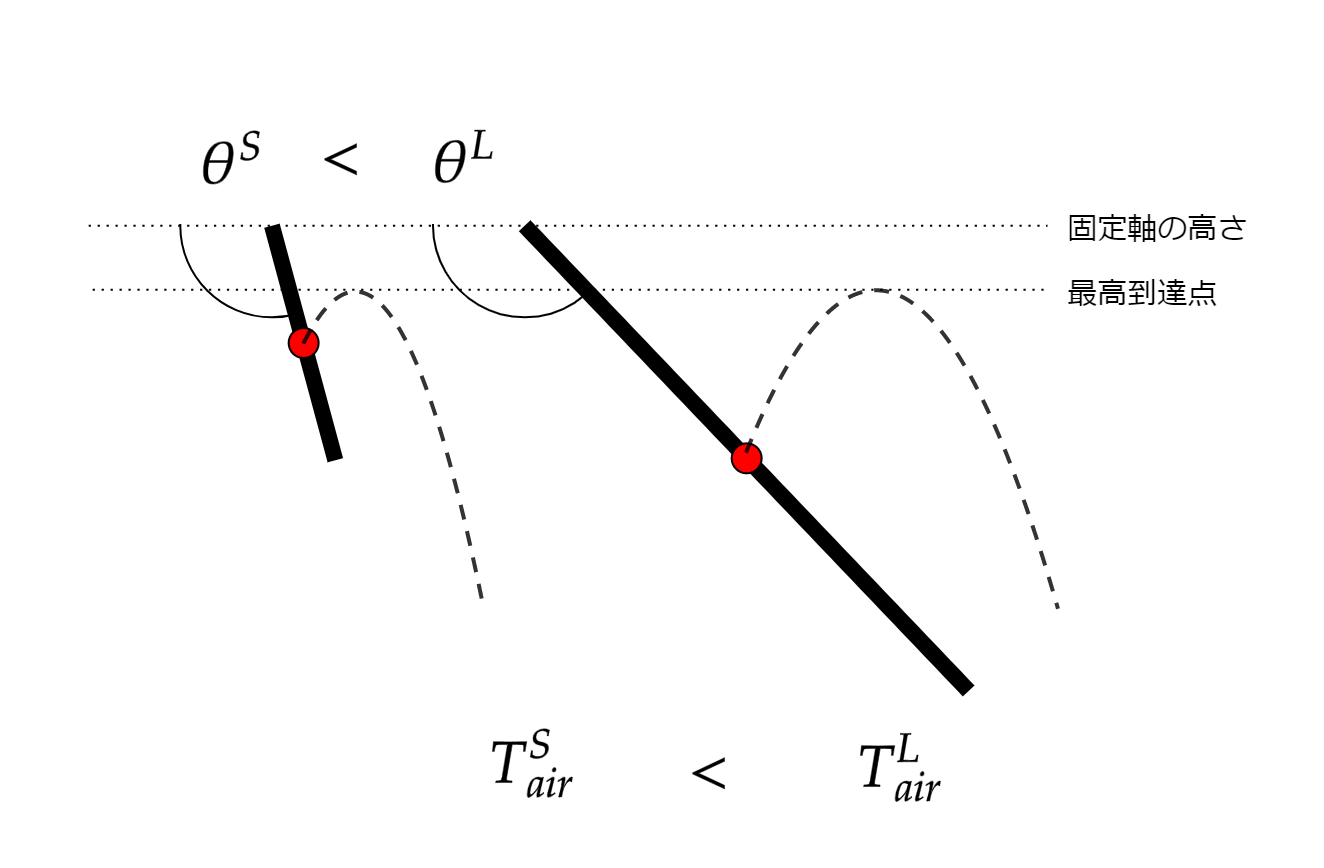
\includegraphics[width = 0.8\textwidth]{same_max_height.png}
  \caption{同じ最高到達点の高度で、長さが異なる振り子の離軸時の様子}
  \label{same_max_height.png}
\end{figure}

最後に空中での回転速度$\Omega$について考える。
$\Omega$は式\ref{eq:Omega}により
\begin{align}
  \Omega^2 
  &= \frac{m^2g}{6I^2}l^3\sin\theta
  \\
  &= \frac{m^2g}{6I^2}\sin\theta \cdot \frac{64(-h^3)}{\sin^3\theta(3\sin^2\theta+1)^3}
  \\
  &= \frac{m^2g}{6I^2}\cdot \frac{64(-h^3)}{\sin^2\theta(3\sin^2\theta+1)^3}
  \\
  &= \frac{32m^2g (-h^3)}{3I^2}\cdot \frac{1}{\sin^2\theta(3\sin^2\theta+1)^3}
\end{align}
と表されるから、
\begin{align}
  l^S &< l^L
  \\
  \Leftrightarrow
  \sin\theta^S &> \sin\theta^L
  \\
  \Leftrightarrow
  3\sin^2\theta^S + 1 &> 3\sin^2\theta^L + 1
  \\
  \Leftrightarrow
  \frac{1}{3\sin^2\theta^S + 1} &< \frac{1}{3\sin^2\theta^L + 1}
  \\
  \Leftrightarrow
  {\Omega^S}^2 &< {\Omega^L}^2
  \\
  \Leftrightarrow
  \Omega^S &< \Omega^L
\end{align}
よって
離軸後の最高到達点の高さが一定であるような条件において
長さ$l$に対して空中での回転速度$\Omega$が単調増加であることが示された。

これによって
離軸後の最高到達点の高さが一定であるような条件において
長さ$l$に対して
離軸時の角度$\theta$、
滞空時間$T_{air}$、
空中での回転速度$\Omega$
が単調増加であることが示された。

適当に着地点の高さを決め、滞空時間が完全に決定される状況にすると、
離軸時の角度$\theta$、
滞空時間$T_{air}$、
空中での回転速度$\Omega$は
図\ref{result.png}のようになる。
\begin{figure}[h]
  \centering
  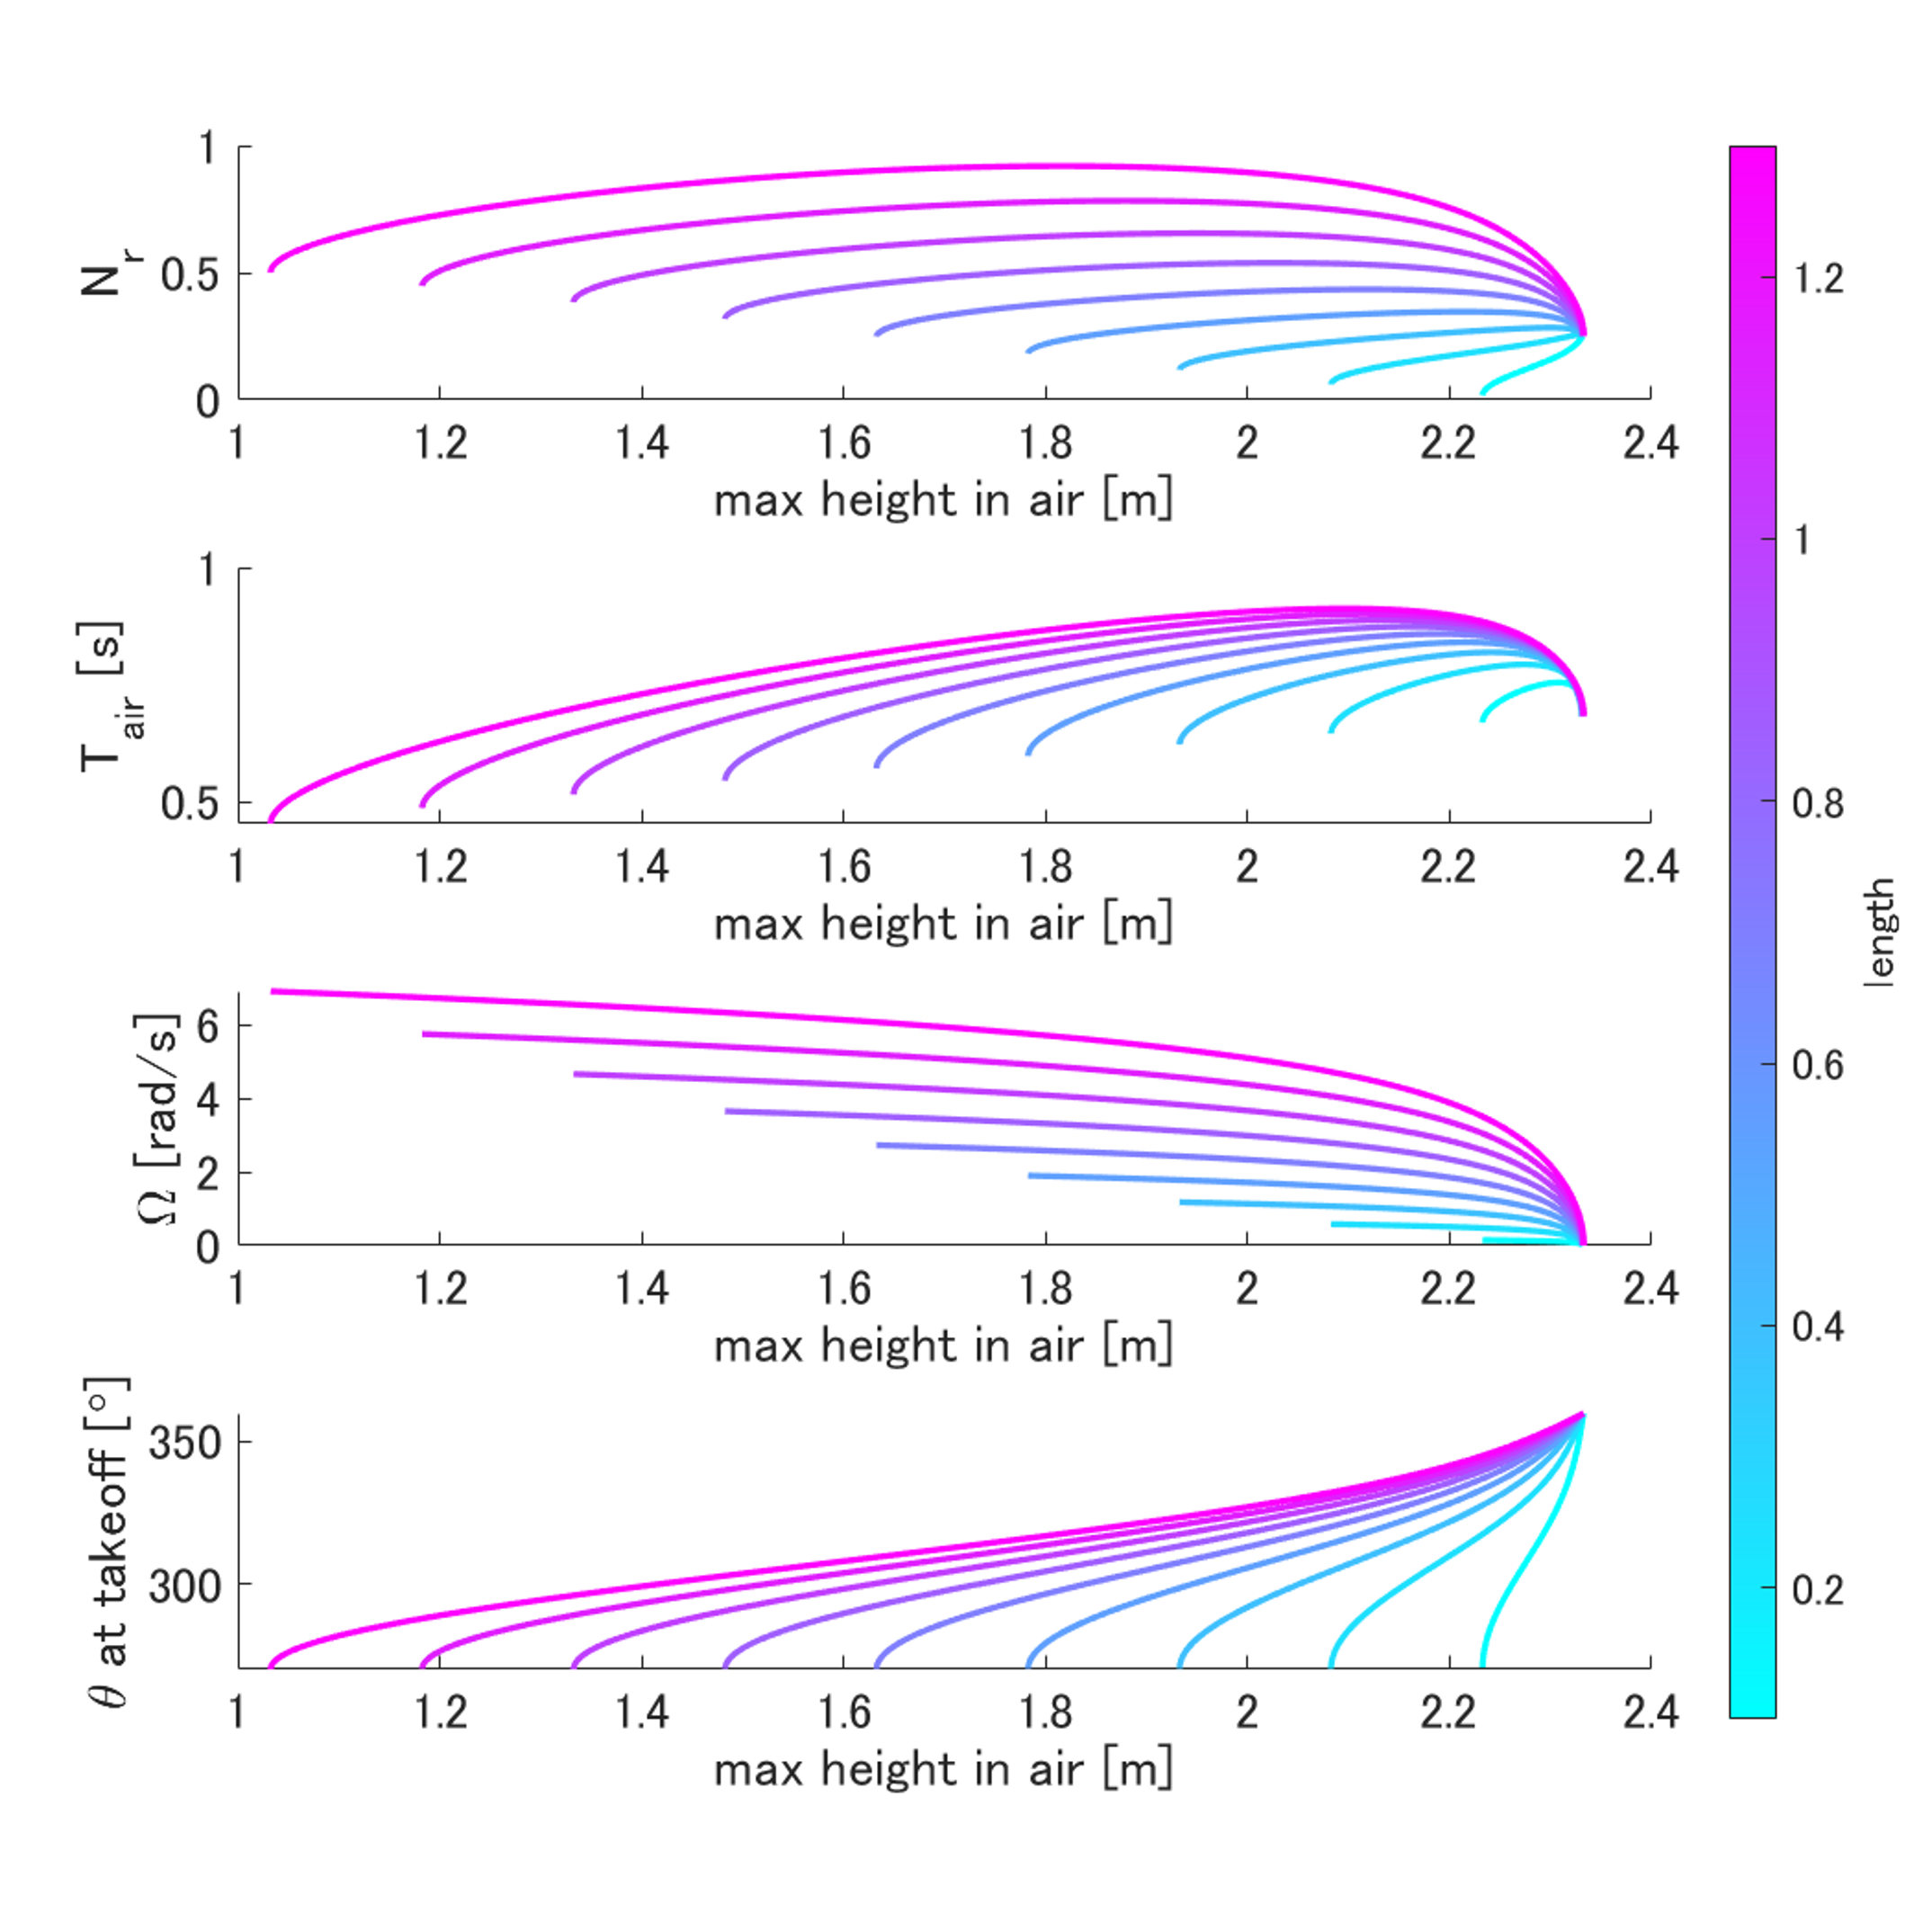
\includegraphics[width = 0.6\textwidth]{result.png}
  \caption{
    実際の
    離軸時の角度$\theta$、
    滞空時間$T_{air}$、
    空中での回転速度$\Omega$
    の様子
    }
  \label{result.png}
\end{figure}

ちなみに、今までの考察によって
各長さに対して最高回転数を与える離軸時の角度は分からない。
解析的にもちろん求められるが、
どの時点を着地点にするかなどによって変わるので、
シミュレーション値だけを図\ref{Tair_Omega_at_maxspin.png}で紹介する。
長さがある程度長い部分に関して滞空時間があまり増大せず、
回転速度が大きくなる様子は
平行棒モデルでも観測された
(図\ref{Tari_Omega_PB.png})
。

\begin{figure}[h]
  \centering
  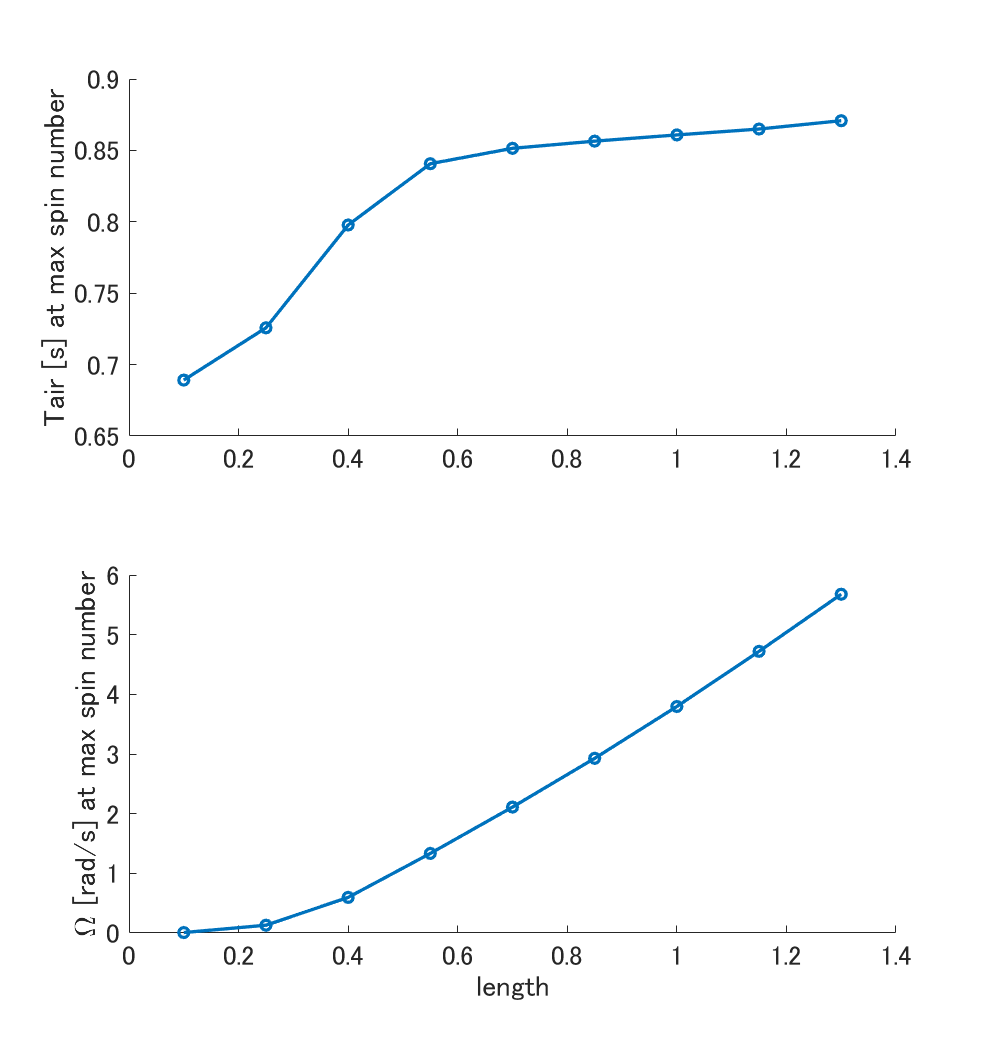
\includegraphics[width = 0.8\textwidth]{Tair_Omega_at_maxspin.png}
  \caption{
    最高回転数を与える離軸時の角度で離軸した場合の
    滞空時間$T_{air}$と
    空中での回転速度$\Omega$
  }
  \label{Tair_Omega_at_maxspin.png}
\end{figure}

\begin{figure}[h]
  \centering
  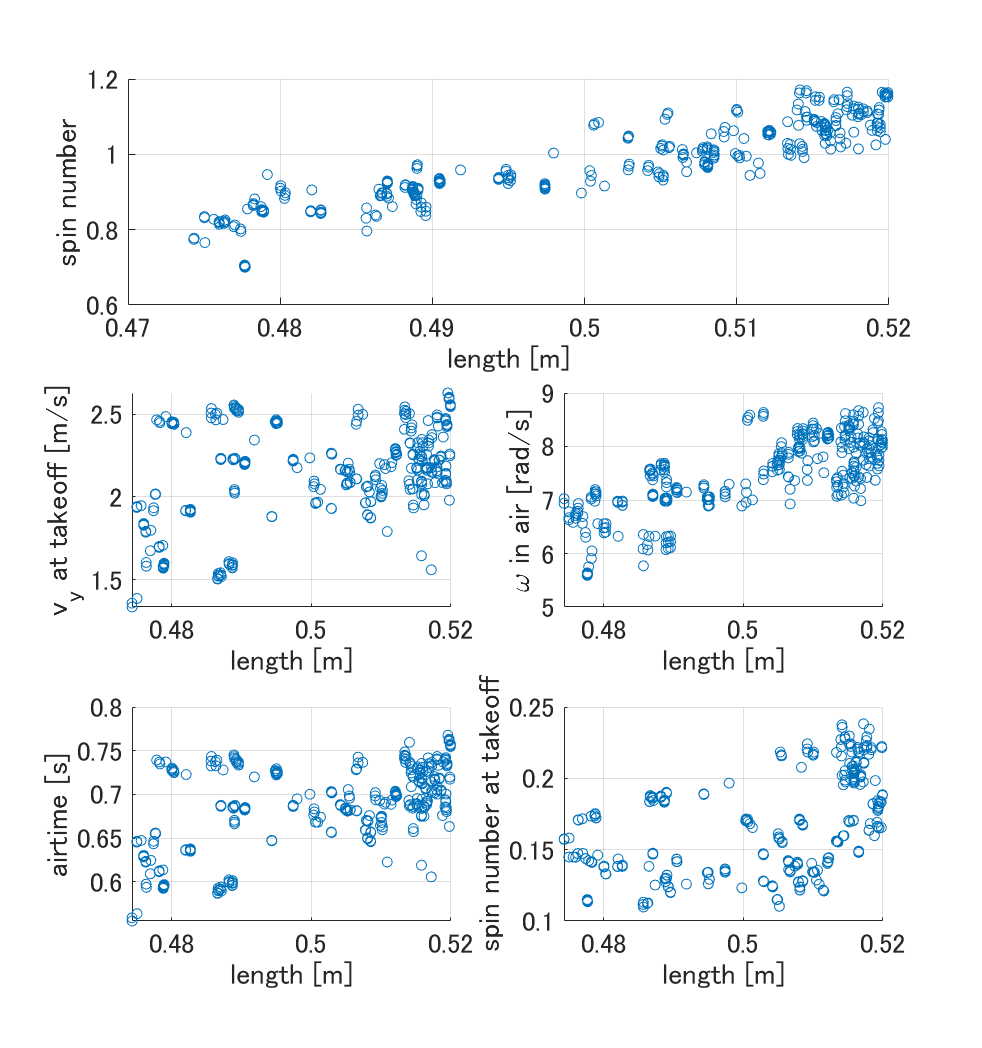
\includegraphics[width = 0.8\textwidth]{Tari_Omega_PB.png}
  \caption{
    平行棒モデルでの
    滞空時間$T_{air}$と
    空中での回転速度$\Omega$
  }
  \label{Tari_Omega_PB.png}
\end{figure}

\end{document}